\chapter{Introduction}

\section{Motivation}
Traditional approaches to data collection often rely on extensive experiments using full-scale systems, such as MilliAmpere.
While these experiments are crucial for specific research purposes, the cost-benefit ratio may not be favorable when the primary objective is to collect sensor data.

The absence of a low-threshold approach to data collection was identified together with my supervisors at the beginning of my integrated Ph.D.
To address this, I embarked on the development of a human-operable sensor rig during my preproject, with the aim of completing it during my \master.
The overarching goal was to create a lightweight \sr that could overcome common challenges like synchronization and pose estimation, paving the way for an accessible approach to low-effort acquisition of high-quality data.


While significant progress was made in the mechanical design and electronic aspects during my preproject, considerable work remained on the software side.
In this \master two key areas were selected as primary focus points.

\subsection{High Speed Video Acquisition and On-the-Fly Compression}
A significant amout of work was put into enabling on-the-fly compression of the videostreams from the \sr.
Each \cam on the \sr features a 5.0MP sensor configured to capture 10-bit raw images 16 times every second resulting in roughly $1Gb/s$ of data \cite{lucidvisionlabsTriton0MPPolarization}.
To put this into perspective, a single frame contains more data than is needed to store the entire collection of William Shakespeare's works in plain text \cite{projectgutenbergCompleteWorksWilliam1994}.
If the output from these cameras were stored directly to disk, almost a Terabyte of data would be generated every hour, making it infeasible to collect long term data sets.
The \gls{imu} and \gls{gnss} also contribute some amout of data, but negligible compared to the cameras.

Simply buying a 8$8TB$ \gls{ssd} was considered and  would enable 9 hours of recording \cite{CorsairMP600PRO}, but several arguments for enabling on-the-fly compression were remained:

% \cite{microntechnologyMicron2300SSD2020}

\paragraph{Limited write speed to the SSD}
One issue when storing the raw data at first was that the \jx is that the \jx is incapable of writing fast enough to the current \gls{ssd} even though the \gls{ssd} is more than capable \cite{microntechnologyMicron2300SSD2020}.
The write speed was tested using the \code{dd} tool
\footnote{\code{sudo dd if=/dev/zero of=./testfile bs=8k count=100k conv=fdatkasync}}
which repeatedly reported write speeds just below $2Gb/s$.
This is weird but other people have faced similar issues on the \jx \cite{dtyuImbalancedPerformanceRead2018}.
This is probably fixable, but is solved by compression.

\paragraph{Streaming to external devices}
Another key benefit of having a compression pipeline in place is that it enables streaming the video feed wirelessly to external devices, at a higher compression rate, for monitoring purposes.
With variable bitrate encoding the video can even be streamed over a 4G/5G connection, enabling remote monitoring of the \sr.

\paragraph{Integration with other systems}
Finally, while the main intended purpose for the \sr is to be used as a standalone system for data acquisition, the design process has been guided by the goal of making it easy to integrate with other systems.
Keeping the total data rate below $1Gb/s$ makes it possible to use the \sr as a sensor module in a larger system, such as MilliAmpere, by connectin it over standard Ethernet.

\subsection{Graphical Web Interface and Ergonomic Improvements}
The ultimate objective for the \sr is to make data acquisition as easy as possible.
Given the significant effort invested, ensuring user-friendliness for individuals without technical expertise in data collection was a priority, as we aim
To accomplish this, a graphical web interface was developed, enabling real-time control and monitoring of the \sr.
This eliminates the requirement for SSH access and transforms the \sr into a plug-and-play system.

The end goal for the \sr is to be carried around by a human operator and used to collect data in a variety of environments.
With the amount of work invested we wanted to make sure that the \sr would be easy to use, also for people without technical expertise in the field of data collection.
In order to acheive this a graphical web interface was developed to enable real time control and monitoring of the \sr, removing the need for any ssh acces, making the \sr plug-and-play.

\subsection{Polarization Cameras}

\begin{figure}[H]
    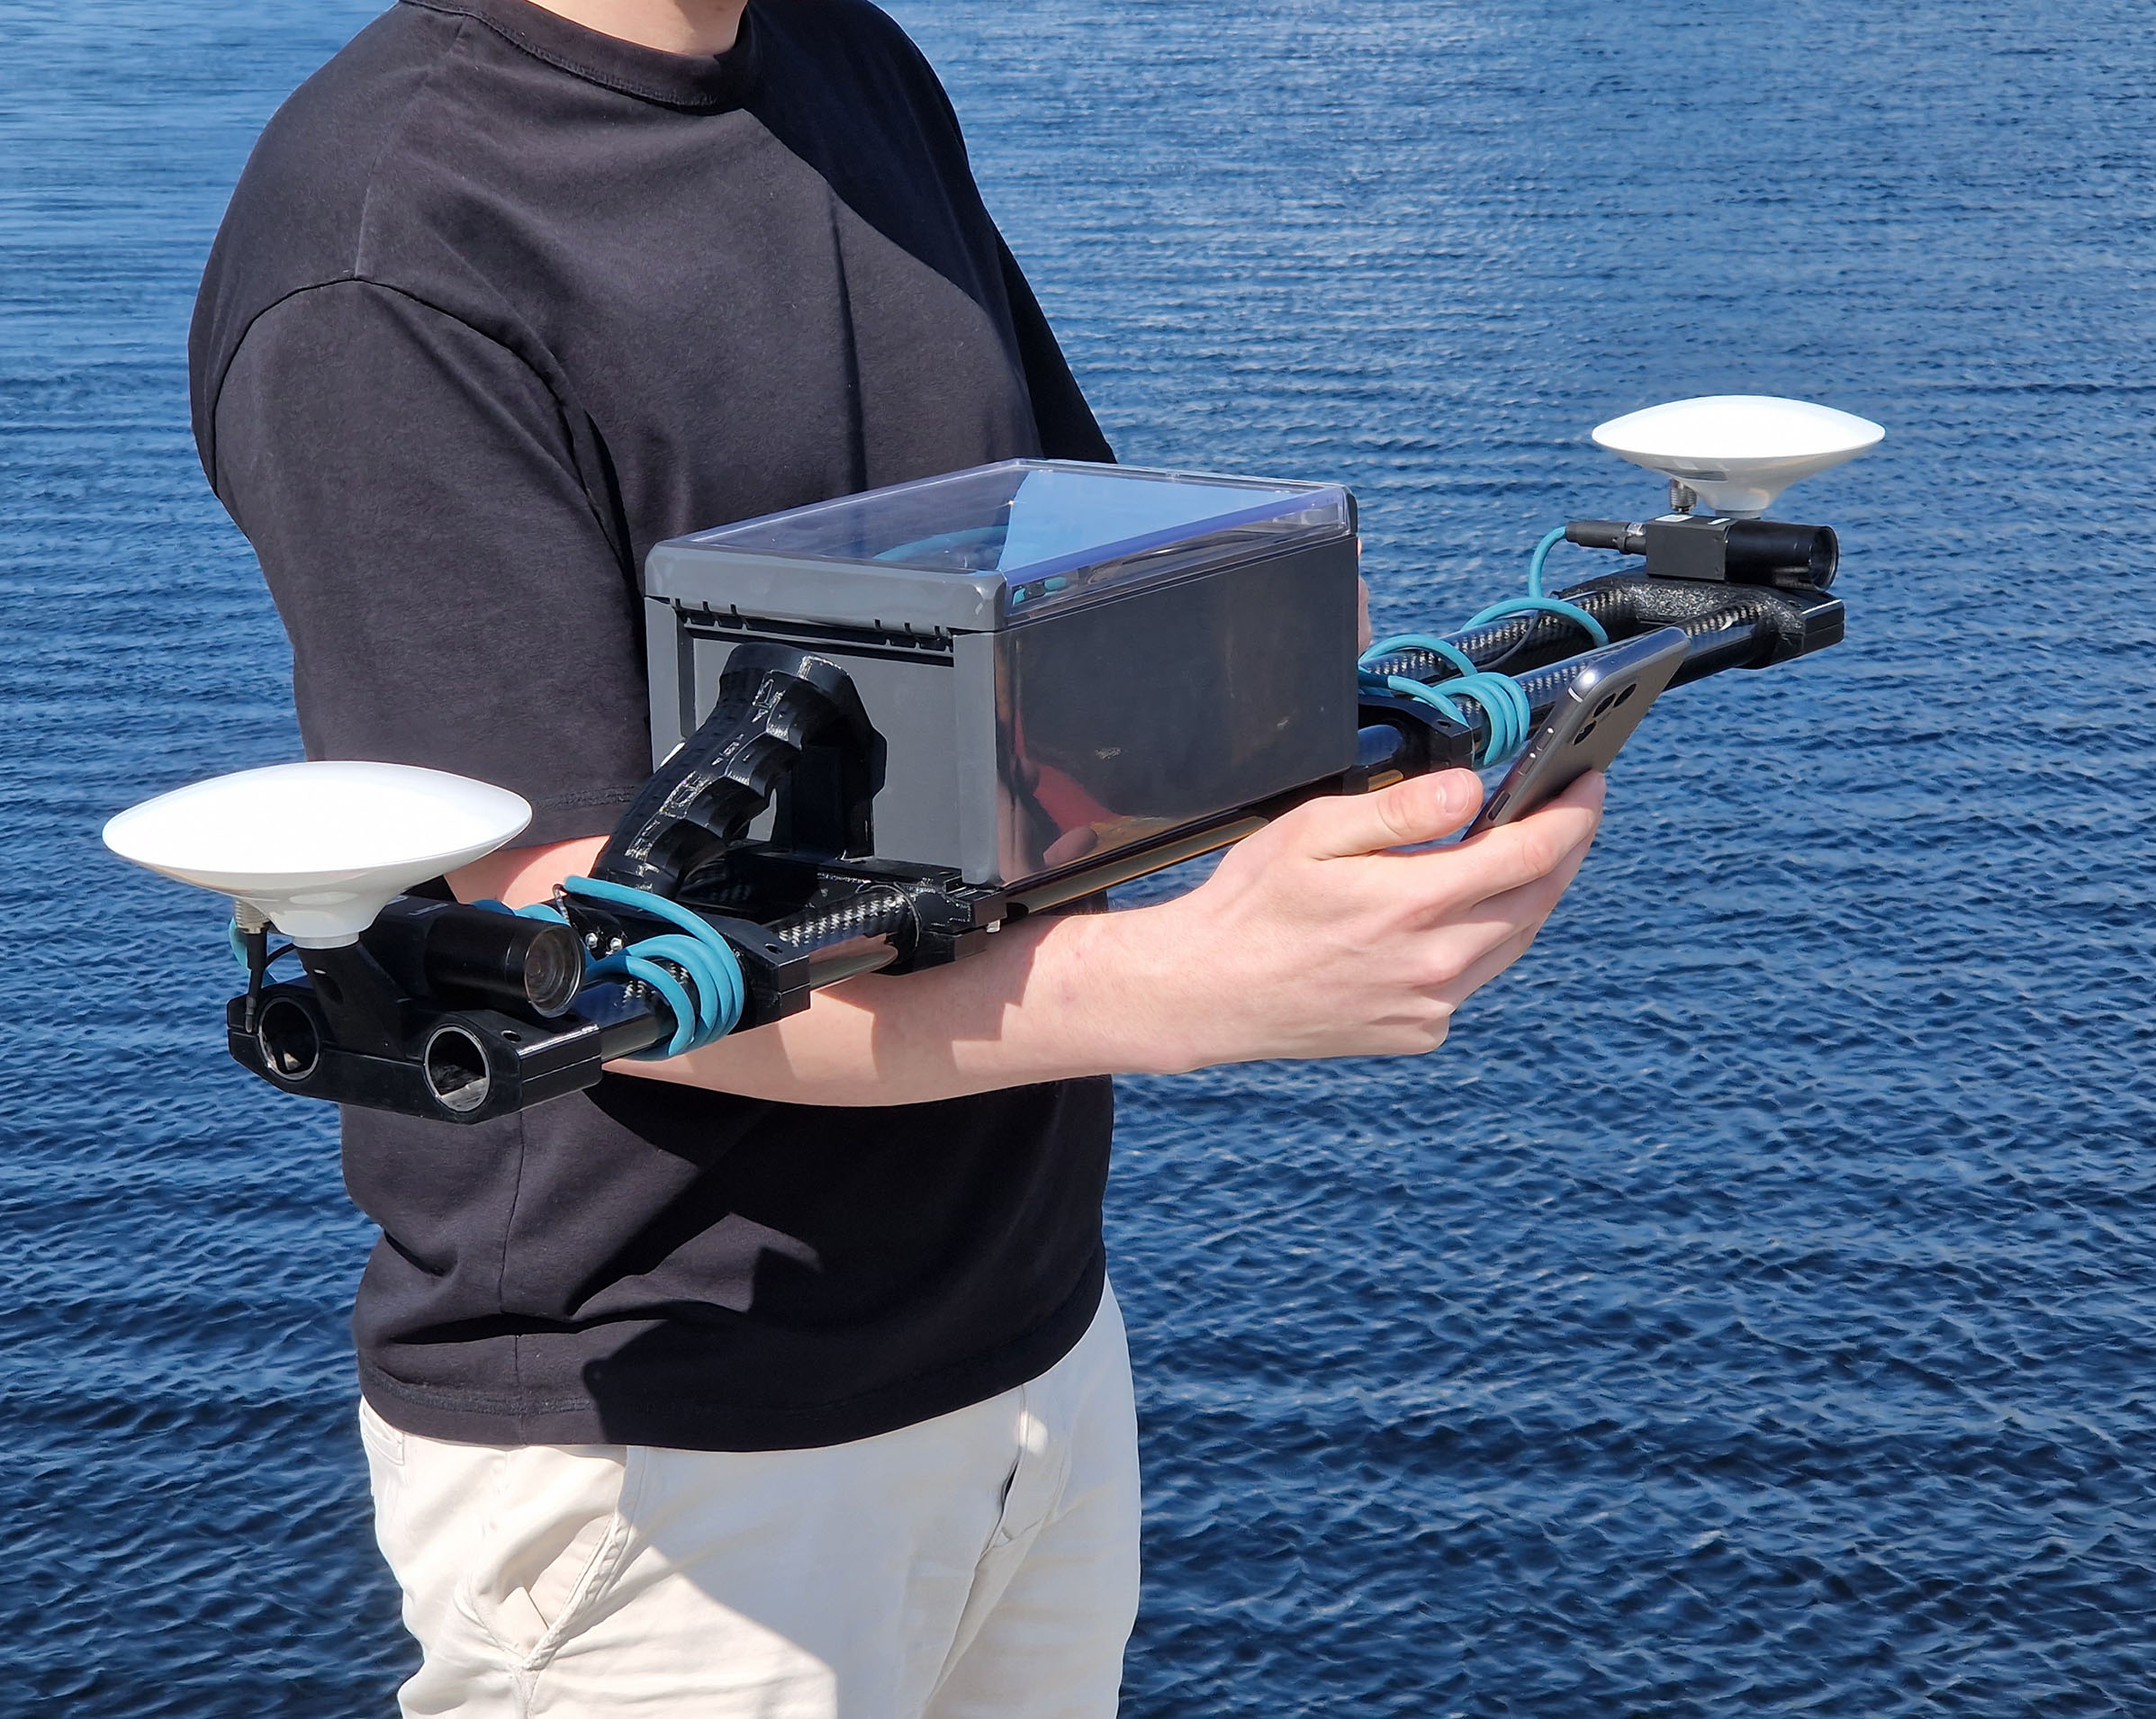
\includegraphics[width=\textwidth]{figures/frontpage.jpg}
    \caption{The Sensor Rig}
\end{figure}

\section{Previous Work}
This \master is an extension of the work done in my \preproject \cite{martensPortableSensorRig2022}.
During the preproject I finished most of the hardware design of the \sr
and assembeled the necesary electronics for \gls{spi} communication between the \jx and the \gls{navbox}, which is the small assembly containing the \gls{imu} and the \gls{gnss} receivers.
Beyond this a solved a several other problems that were encountered, including figuring how \gls{ip67} rating could be acheived.

At the end of the \preproject the \sr was capable of collecting data from the \gls{imu} and the \glspl{gnss} and validate the \gls{crc} checksum on the incoming data, but I har not implemented
I had verified that it was possible to read data from the \cams over the ethernet interface, but only a at a very low framerate using the default settings.

As this \master is closely related to the \preproject it will reference several sections and figures to avoid having to repaeat wats already written there and the reader is advised to have it available.

\section{Main Contributions}
The main contribution of this \master is the delivery of a working \sr capable of recording high quality stereo polarization datasets.
Working with real hardware constantly introduces unexpected issues and overcoming these in a systematic manner has been a major part of the work.
In terms of specific techical achievements the following are the main contributions:

\begin{itemize}
    \item Developed and implemented a higly efficient CUDA kernel transforming the raw output from the \cams into the widly used \gls{p010} format.
    \item Assembled a \py acessible \gls{gstreamer} pipeline for hardware acceleraded compression on the \jx.
    \item Developed a fulstack graphical web interface acessible from mobile devices.
    \item Designed and 3D-printed ergonomic handles for the \sr.
\end{itemize}


\section{Outline}
Completing the \sr project has involved extensive work on various topics, ranging from hardware design and full stack web development to kernel compilation and low-level optimizations in CUDA.
Although some of the topics are closely related, others are only connected  by contributing towards the final product.

With this in mind it has been difficult to decide on a structure for this report and what to include.
In the end I decided to collect the software development theory in the first chapter, and dedicate a chapter to each of the major topics I have worked on with a focus on the practical aspects of the work, to serve as a referece for future work.

As some chapters might be less relevant depending on the reader's background, I have tried to make each chapter as self-contained as possible.
Figure \ref{fig:overview} provides an overview of the chapters in this \master and how they are connected.
The following is a brief overview of the content of each chapter:

\begin{figure}[H]
    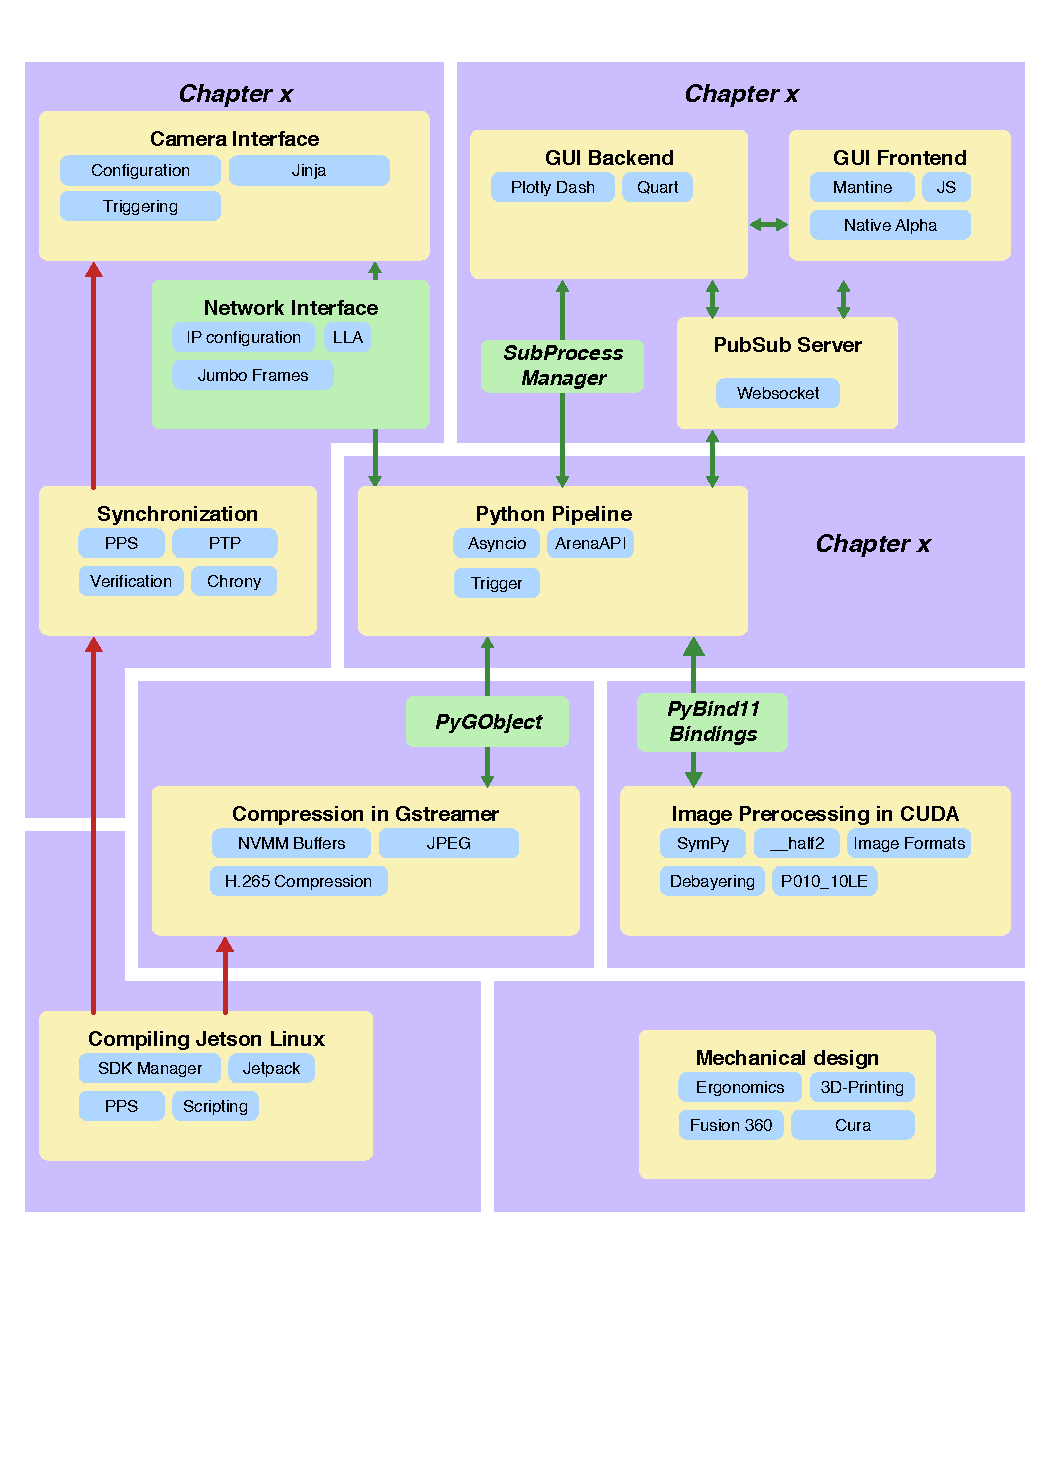
\includegraphics[width=\textwidth]{chapters/10_intro/chapter_overview.pdf}
    \caption{Overview of the chapters in this \master.}
    \label{fig:overview}
\end{figure}


\paragraph{Chapter \ref{chap:programming_theory}: Real time programming on Jetson Xavier}
This chapter provides an overview of the theoretical background relevant to real-time performance on the Jetson Xavier platform and the development of real-time software in general.
It explores topics such as real-time programming theory, performance considerations for heterogeneous systems, and introduces the CUDA programming model.

\paragraph{Chapter \ref{chap:cameras}: Polarization Cameras}
This chapter presents the special type of polarization cameras used, explain how they work and why they are particularly well suited for detection in marine environments.
Furthermore, it covers how to interact with the \cams through thair \gls{api} and how the network adapters have been configured to acheive reliable $2Gb/s$ throughput from the \cams.

\paragraph{Chapter \ref{chap:debayer}: Efficient processing of raw image bitstream in CUDA}
To make it possible to compress the video streams, the raw data has to be transformed into a format that can be processed by the \gls{h265} encoder.
This chapter explains how this is acheived in real time using CUDA.

\paragraph{Chapter \ref{chap:gstreamer}: Video Compression using GStreamer}
\gls{gstreamer} is a powerful framework for processing video streams.
This chapter explains how it is used to compress the video streams in real time using hardware accelration on the \jx.
It also covers how \gls{pygo} is used to interact with the \gls{gstreamer} pipeline from Python.

\paragraph{Chapter \ref{chap:pipeline}: Pipeline Assembly in Python}
The three previous chapters are tied together in this chapter, which explains how the various components are assembled into a working pipeline.

\paragraph{Chapter \ref{chap:gui}: Web Interface to Control, Monitor and Stream Video}
A web application was developed to enabling real time control and monitoring of the \sr and its video streams.
This allows anyone with a smartphone to operate the \sr without any prior training or technical knowledge.
In a ddition a \gls{pubsub} server was implemented for communication between the web application and the pipeline.

\paragraph{Chapter \ref{chap:flashing_xavier}: Compiling Jetson Linux with PPS}
This chapter presents a systematic approach to compile, flash and debug the \gls{os} on the \jx.
Updating the \gls{os} was necessary to get the \gls{gstreamer} pipeline working.
As a \gls{pps} suuport is requiered  to synchronize the clock on the \jx to \gls{utc}, it was necessary to configure the underlying Linux kernel to support this, which was more complicated than expected.

\paragraph{Chapter \ref{chap:hardware}: Improving the Hardware}
After the \preproject most of the hardware was already in place, but some parts were missing.
I applied for, and got, funding to purchase a new 3D printer to enable an iterateive design process.
With this in place custom ergonomic carry handles, new combined camera and antenna mounts and other minor parts were designed and 3D-printed.

\paragraph{Chapter \ref{chap:results}: Results}
With everything in place, the \sr was tested in the field.
Several smaller datasets are collected and visualization tools has been developed to facilitate analysis of the data.

\paragraph{Chapter \ref{chap:future_work}: Ongoing developments and future work}
Some design flaws from the \preproject remain to be fixed and a few possible performance improvements have been identified.
With the goal of creating a fully autonomous sensor rig acheived, the next step is to create state of the art stereo polarization datasets and advance the field of situational awareness for autonomous surface vessels.

